\newpage
\section{Implementation}
This chapter presents the implementation of the newly created design system as a standard for the web user interfaces for SaaS products. \\
First, a look at the architecture and modelling is taken. Looking at existing design systems and trying to understand  how they work and extract requirements in order to develop a common system that fits most products in the SaaS world. \\
After that this chapter presents an actual implementation of a component, including the technology stack used and how the components are built. \\
Finally, the build chain is explained. Including all information on how components and atoms are consumed and bundled. Also giving an outlook what is needed to get the SDS running inside a existing or new project.
\subsection{Architecture}
Modelling the architecture of a system that supports customization of SaaS product user interfaces is not a trivial task. Often, user interfaces for products are developed only to support their purpose. Finding common ground for multiple products can be difficult.  \\
Design systems define a common place where the company's products can align. Why is it not possible to develop a central system to create a common idea for user-friendly SaaS products? Not only do well-designed components help align, but a design system foundation with guidelines and principles helps developers and designers create a good product. \\
To this end, 10 different design systems of well-known SaaS products, as well as design systems with a shared purpose, were considered. 
\begin{table}[!ht]
\begin{tabular}{|p{0.2\linewidth} | p{0.7\linewidth}|}
\hline
 \textbf{Name} & \textbf{Description} \\ \hline
Service Now  & Platform design system.  Guidance to create components and upload them to the platform. \\ \hline
Adobe Spectrum  & User centralised design system. Many well designed components with matching guide to deliver a great experience. Built in web components and react components. \\ \hline
Zendesk Garden & Basic design system with guidelines, components and patterns. Tailwindcss integration. Built in react components. \\ \hline
Atlassian Design System & Design System connected with company values. A lot of guides on how to use designs, components and to write content. Includes also employee motivation. Built in react components. \\ \hline
Base Web  & Open source design system. Used by Uber. Providing a blog and guides on how to use the base design system. Design System intended to be used as baseline and should be overwritten when used. No principles or values included. \\ \hline
SAP Fiori  & Standard design system. Focus on accessibility and multiple device support. Including many themes for different applications. Delivers a toolkit to better use the design system as a designer.  \\ \hline
GOV UK Design System  & Not really a design system. Missing guidelines and principles. Externals can propose changes. Providing CSS classes for HTML elements.  \\ \hline
Lightning Design System & Design System to support developers and designer at their work. 4 principles with a clear message to align every user. Guidelines and best practices on many topics.  Components are built with pure CSS classes. \\ \hline
Google Matrial Design & Open source design system. Providing the user with design principles which helps to understand the usage of the design system. Material Design provides only components and no patterns. Blogs and further resources are helping additionally to the guidelines. Components are built with pure CSS classes. \\ \hline
Pluralslight Design System & Design System without principles and guidelines. For the moment only components are present. Providing a workflow for developers and designers to contribute to the design system.  Only few patterns. Built with react components.  \\ \hline
\end{tabular}
\caption{\label{tab:design_systems_in_the_wild} Overview of 10 existing design systems}
\end{table}
As can be seen in table \ref{tab:design_systems_in_the_wild} fot these 10 examples of design system, the interpretation of one can vary. \\
A good reference for a design system with a suitable use case is the Base Web Design System. Its purpose of providing a base of styles and functional components helps developers customise for their products. Also, the fact that this design system is open source underlines that this design system has been developed by the community and is not controlled by a corporate design team. Built-in accessibility is also a requirement that must be present in a common design system. The instructions on how to extend and use the design system are also a perfect reference. \\
But there are also disadvantages. The Base Web Design System lacks guidelines and principles that are crucial for a design system. A look at Google's Material Design shows that even an open-source and versatile design system can have design principles. Design principles help developers get an idea of how to develop and design with the system. Therefore, design principles are indispensable in a design system and should not be missing. \\ \newpage
Another reason, is the use of React for creating the components in the Base Web Design System. As a design system that should be used by everyone as a standard for the implementation of SaaS products, it is therefore unsuitable. As developers are expected to use React as a frontend library. Looking at other examples such as the GOV UK Design System or Salesforce's Lightning Design System shows that it is possible to create components using web standards that can be used by anyone without having to use a library. \\
With these requirements, an architecture can be drawn as can be seen in figure \ref{architecture_sds}. \\
\begin{figure}[htbp]
\centerline{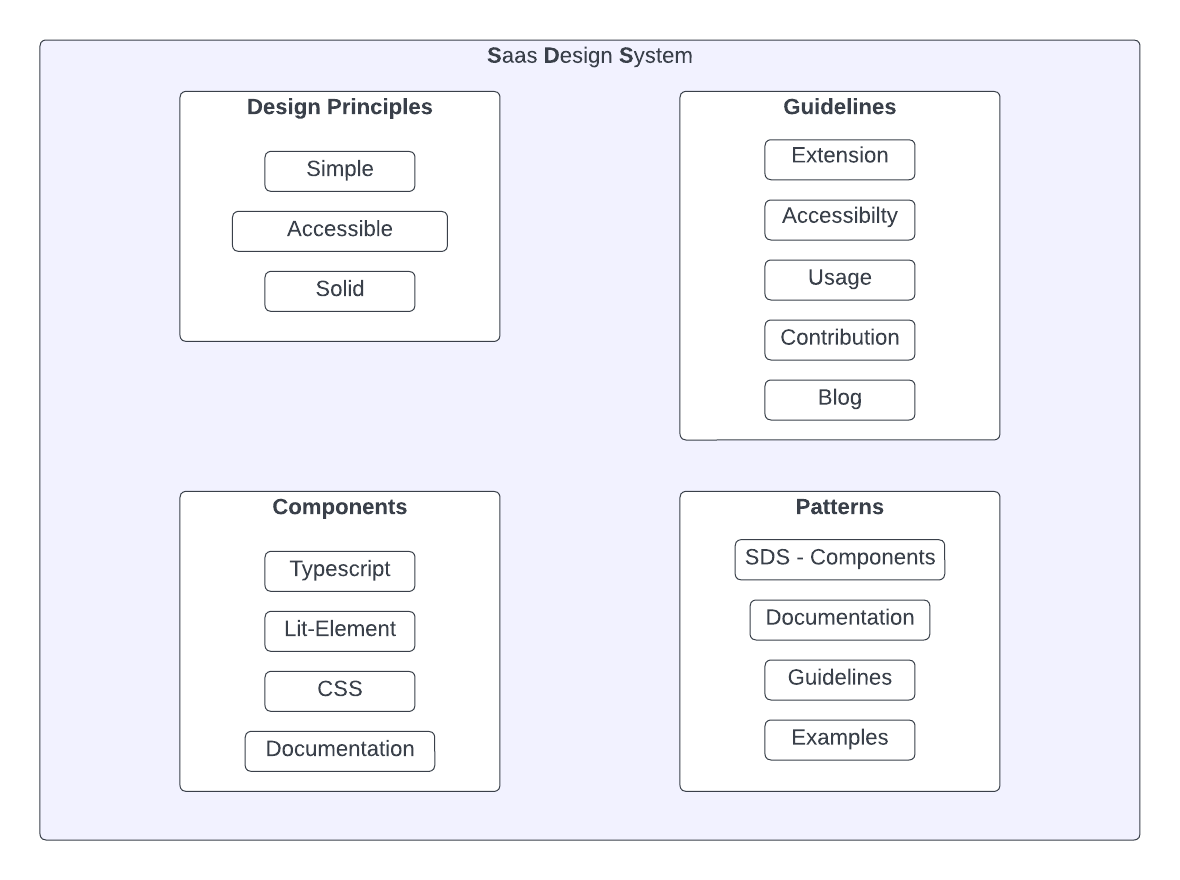
\includegraphics[width=\linewidth]{images/architecture_sds.png}}
\caption{Architecture of SaaS Design System}
\label{architecture_sds}
\end{figure}
According to the description of a design system presented in chapter 2, the SaaS design system can be roughly divided into four parts.
\subsubsection*{Design Principles}
In terms of design principles, the SDS strives to keep them lean and easy to understand, as the design system is intended to serve as a basis for other design systems. The \textbf{Simple} principle states that component design should not have unnecessary styles or features that make it difficult to extend. \\
Many products strive to implement accessibility in their products. With the \textbf{Accessible} principle, SDS emphasises the importance of accessible user interfaces. This is not only important in terms of inclusion, but also helps accessibility in the overall user experience for all users. \\
The third and final principle is \textbf{Solid}. As stated earlier, the SDS should be a foundation for other design systems to build upon. Therefore, the importance of a stable and consistent API is very important. For this reason, the design system has deliberately chosen \textbf{Solid} as the third and final principle. \\
\subsubsection*{Guidelines}
The SDS guidelines are based on the design principles just presented. In addition to the core guidelines on extension, accessibility and basic use, there are also guidelines that focus on contributions and collaboration. As this is an open source system, as many people as possible should be able to work on it. \\
The extension guidelines address how to integrate SDS as the basis for a company's own design system. It shows developers and designers how to create their own from the components provided. \\
Since accessibility is also a design principle, there must be a guideline that defines what the SDS means by accessibility. It should give the user a definition and sources for accessibility. But also self-designed components should have a guideline that helps users to implement accessibility. After this guideline, the user should have no more questions about accessibility. \\
As a third guideline, the SDS will support the user in using the system. This guide could also be seen as an entry guide and will cover the basics. Importing the design system, proper bootstrapping and guidance on configuring the system. This may seem self-explanatory, but lacking these often prevents users from using the system effectively. The user guide should be as simple as possible and cover every small step needed to get started with the SDS. \\
One goal of this design system is to be developed by the community for the community. However, this can quickly get out of hand if everyone contributes without any guidance. Therefore, it is important to introduce some from the beginning. This guide provides guidance on how to contribute to the component library, but also on how to enforce changes to the guidelines and principles. As this design system is not set in stone, there should be opportunities to change and adapt everything. What this will look like in the end will evolve over time. Some ideas could be a voting process or an RFC (source) process, as is common in the software industry. \\
To achieve high interactivity in such a design system, some design systems introduce blogs and forums for knowledge exchange. In this way, users can connect, discuss and contribute to ideas to further improve the design system. The most important point is the moderation of such an interaction platform. A well-moderated blog and forum will further enhance the community around the SDS. \\
Overall, it can be said that the guidelines for the SDS are aimed at building a community around the design system to contribute and enable users to create a community design system. 
\subsubsection*{Components}
Without well-assembled components, design systems cannot exist. Therefore, choosing the right technology package for building components is very important. 
In the case of SDS, one of the most important requirements is that the system is usable independently of the front-end framework used. To achieve this, SDS uses the web components that are supported in almost all modern browsers. As it is possible to create web components without importing libraries or frameworks, it is a perfect complement for SDS. (Source)\citep{component_definition} \\
Creating web components natively can be complicated. For this reason, the Lit framework was designed to make it easier for developers to create web components. With a focus on ease of understanding, intelligent DOM updates and small package size (5 KB), Lit is a perfect complement for creating components for design systems based on standard web components. \citep{component_definition} \\
To further assist developers, SDS uses Typescript, a superset of Javascript. It extends Javascript with types and interfaces. Typescript must be compiled into Javascript for the browser to understand it, but this allows the developer to find errors much faster because it fails at compile time rather than at runtime. \citep{component_definition} \\
To use and provide design tokens for colours or spacing, the SDS uses custom CSS variables. They are imported into the root element during bootstrapping of the design system. The definition of the design tokens can be found in the documentation. \citep{component_definition} \\
Last but not least, the design system components created must be documented and accessible to users. To start SDS, Storybook is used, which has a lot of built-in functions that support documenting the components. With MDX, the combination of Markdown templating (MD) and code injection via JSX, it is possible to write fluid documentation without having to jump back and forth between files. \citep{component_definition} \\
With this technology stack, SDS provides users with highly reusable web components that are not only easy for users to access, but also easy for contributors to develop. 
\subsubsection*{Patterns}
An essential part of the SDS are the patterns. They describe how user interfaces should be designed to align with the core capability of this design system. The patterns help developers automatically apply best practices and web standards without having to read an entire text. \\
Patterns are created using components and standard HTML elements provided by the design system. These are easily accessible to the developer by copy and paste. With additional documentation on when to use them and when not to use them. \\
The patterns are supported by additional guidelines on how they can be adapted and redesigned. This enables developers to meet the requirements needed for their own design system.\\
Accordingly, live examples show the developer how the patterns will work in the final product. With several different examples for each pattern, the possibilities for customising each pattern are presented. SDS users also have the opportunity to share their creations and application of patterns below the documentation. 

\subsection{Design System Components}\label{sds_button}
An important part of the implementation of a design system are the components. As described in chapter \ref{sds-component}, the components are created using the Lit framework. To see a complete example of a component constructed with design tokens and documented with the storybook, the example of the button component of the \ac{SDS} is presented in this chapter. \\
The components use TypeScript to take advantage of custom decorators. The decorators provided by Lit further simplify the boilerplate code for creating a web component. \\
\lstinputlisting[linerange={1-4},firstnumber=1,caption={Initialization of \ac{SDS} button component},label=ButtonInit]{../Code/src/components/button.component.ts}
In listing \ref{ButtonInit}, the component is initialised with the \texttt{@customElement} decorator by passing the tag name as a string and appending it to an \ac{ES6} class. For it to work properly, the class must extend the Lit Element class. When everything has been implemented as described, the web component is registered and can be used with the defined tag, in this case \texttt{<saas-button>}. \\
In order to see something when the web component just created is used, it must implement the render method. This method expects a \texttt{TemplateResult}. 
\lstinputlisting[linerange={19-26},firstnumber=19,caption={Rendering of \ac{SDS} button component},label=ButtonRender]{../Code/src/components/button.component.ts}
Lit element provides the import of a \texttt{html} string literal that can be used to construct the \texttt{TemplateResult} expected by the render function. With this functionality, Lit provides an efficient way to respond to variable changes and intelligently update the \ac{DOM}. \\
Properties also make use of custom decorators and declare properties on web components by writing \texttt{@property} in front of a class attribute (line 19-20, Listing \ref{ButtonRender}). Thus, Lit Element implements change detection and adds automatic type conversion. For a detailed description of the capabilities of this decorator, see the documentation. Whenever the property value of the created button web component changes, the constructed template string reacts to these changes and updates the displayed template accordingly. \\
Last but not least, the web component must use the defined design tokens. Since these tokens are defined by \ac{CSS} variables, they can simply be consumed as follows: 
\lstinputlisting[linerange={5-20},firstnumber=5,caption={Styles of \ac{SDS} button component},label=ButtonStyles]{../Code/src/components/button.component.ts}
The Lit Element framework implements a static property of the \texttt{styles} to its classes. To make it work properly, a string literal \texttt{css} is used to convert a string into the required \texttt{CSSResult} type. In this way it would be possible to consume design tokens via input properties, but to simply manipulate design tokens in one place, the components of \ac{SDS} will use \ac{CSS} variables. In this way, it is possible to customise certain tokens throughout the design system by adapting these tokens. Each component in the \ac{SDS} will use the defined tokens. Line 7-9 in listing \ref{ButtonStyles} shows an example of the use of design tokens for the button component in the \ac{SDS}. \\
Finally, the button component is displayed in Storybook, the documentation tool for \ac{SDS}. Limited to the time frame of this elaboration, the documentation is kept short. Figure \ref{storybook_button} is an example of what the documentation of \ac{SDS} components may look like. A full version of documentation as in other mature design systems will have to be added in a subsequent development of \ac{SDS}. \\
\begin{figure}[htbp]
    \centerline{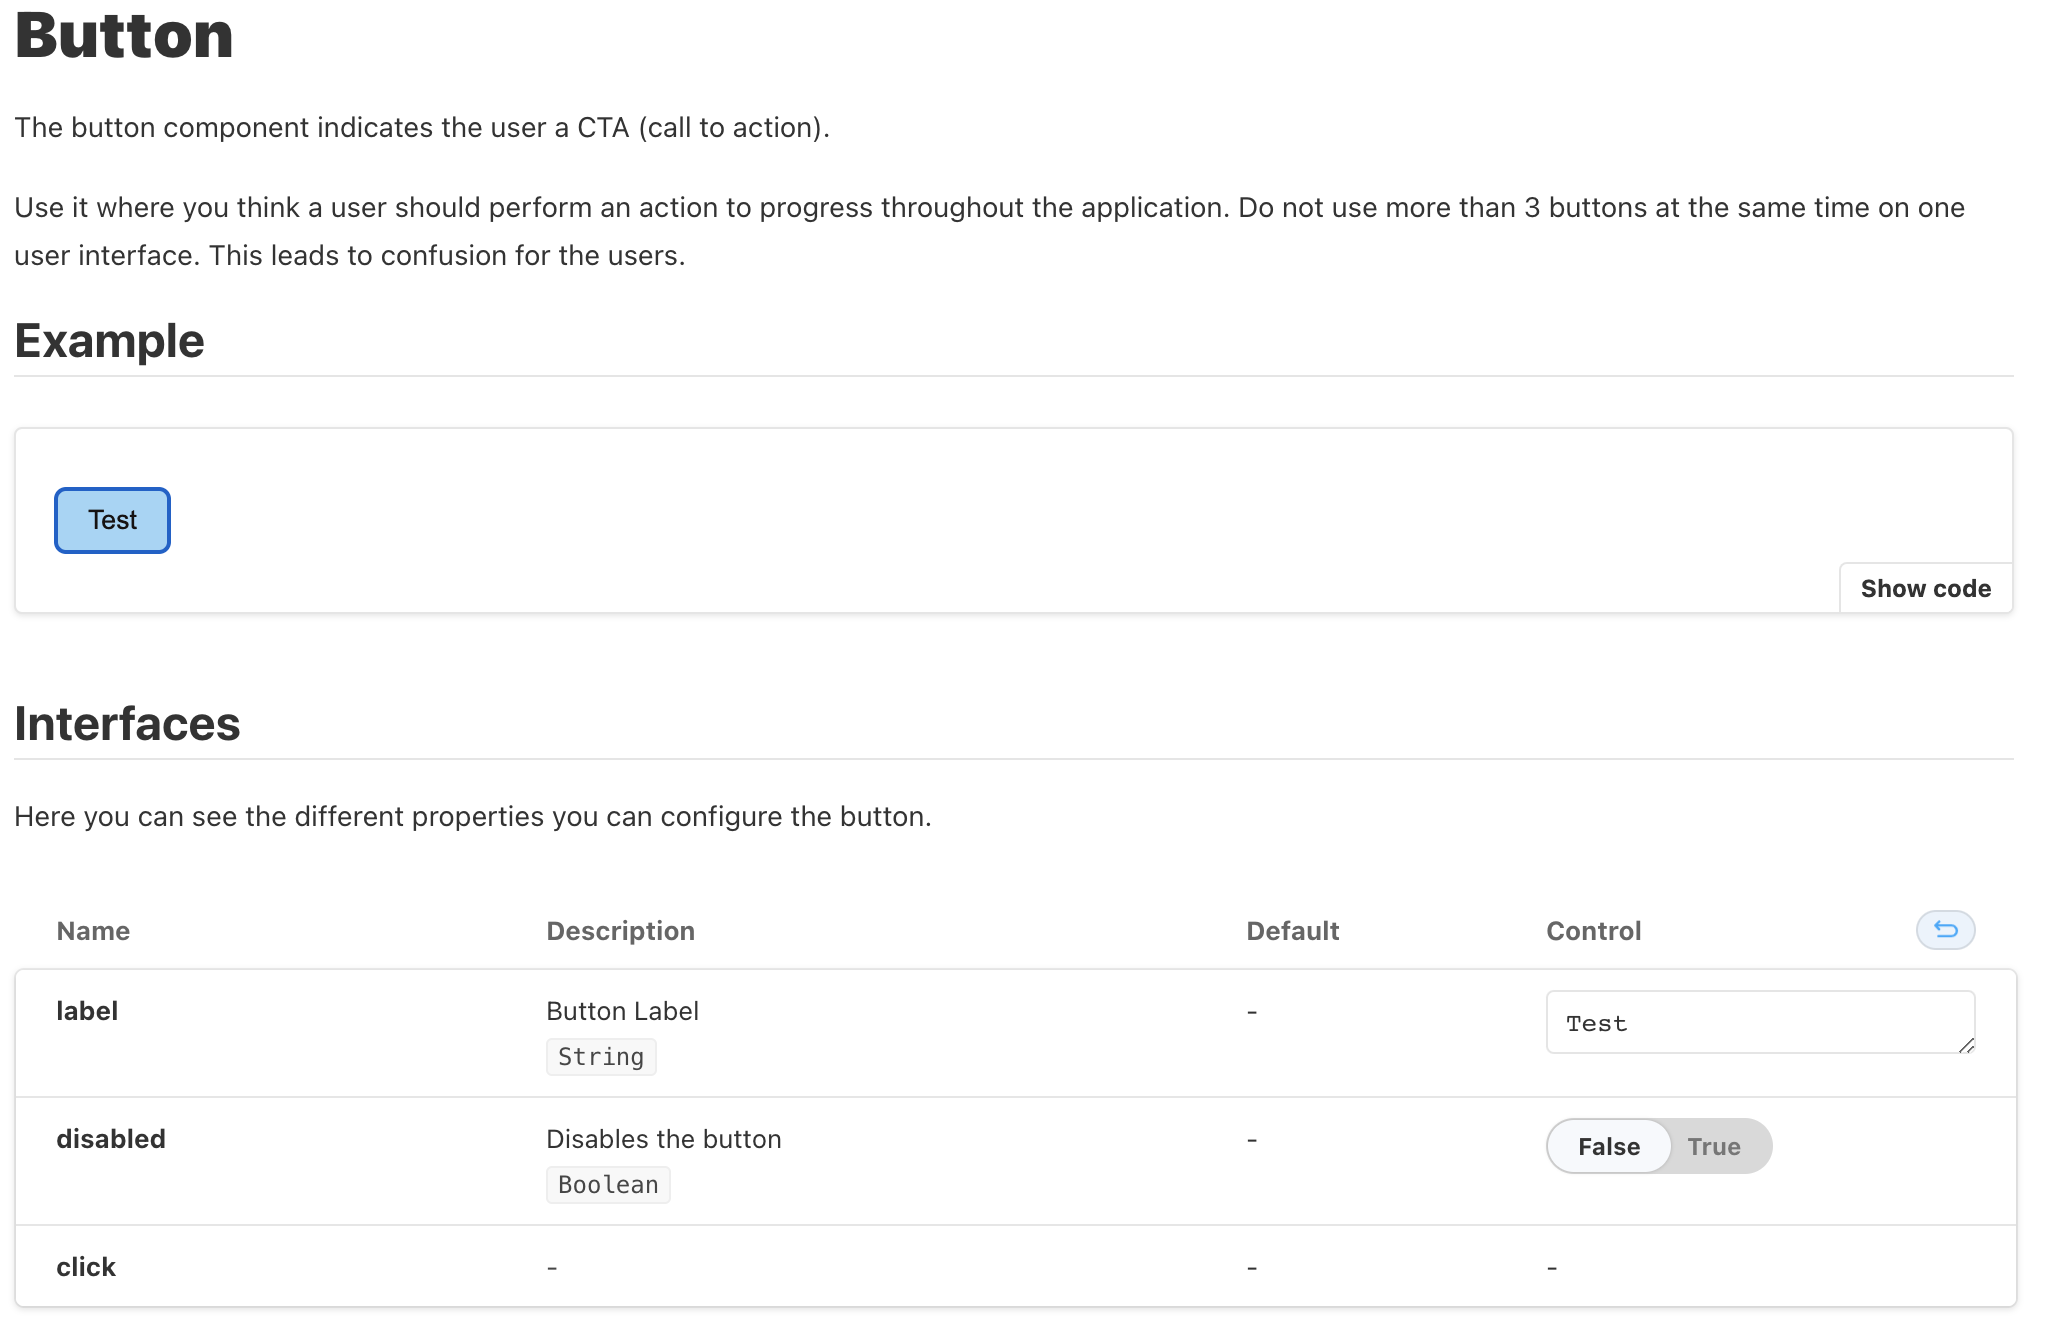
\includegraphics[width=\linewidth]{images/storybook_button.png}}
    \caption{Example documentation of the \ac{SDS} button component}
    \label{storybook_button}
\end{figure}
At the moment, the documentation consists of a short description that briefly explains to the developer how and where he can use the button in his applications. In addition, a live example of the component is presented, which is automatically linked to the properties shown below. When the properties are changed, the example above is updated. This means that the developer or designer who wants to use this component can find out which configuration is most suitable for his use cases. \\
Inspecting the \ac{DOM} element of the button component, the element explorer looks like Figure \ref{button_element_explorer}. When you create a new web component, the saas-button tag is a valid \ac{DOM} element. A new shadow root is opened inside the button component. This allows the web component to isolate styles and elements from the global document. The elements used to display the button component are defined in this shadow root. Also, the styles for the button are defined at the shadow \ac{DOM} level, so the rest of the \ac{DOM} tree never receives these styles. This helps to keep elements and styles separated and easy to understand. \\
\begin{figure}[htbp]
    \centerline{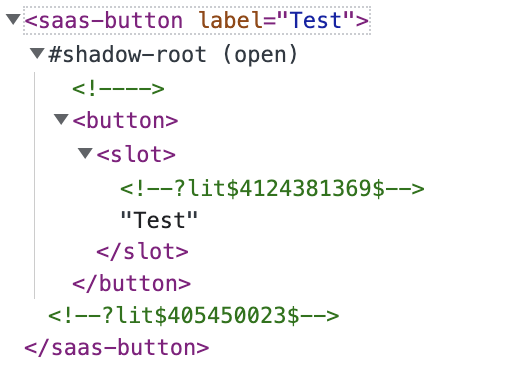
\includegraphics[height=100px]{images/button_element_explorer.png}}
    \caption{Inspection of \ac{SDS} button in elelement explorer}
    \label{button_element_explorer}
\end{figure}
It is important that \ac{CSS} variables declared in the root of the document are also available in the shadow \ac{DOM}. In contrast, style declarations, e.g. for the button element in the overall document, are not applied to \ac{DOM} elements in the shadow \ac{DOM}. \\
The \texttt{<slot>} element in the shadow \ac{DOM} is a default placeholder for anything that is inserted into the \texttt{<saas-button>} element when using the web component. The content is projected within the shadow \ac{DOM} and inserted in place of the \texttt{<slot>} element. This makes it possible to create nested elements with web components which is useful in many different use cases. \\

The example of a simple button component shows how to create and use the components of \ac{SDS}. From here it is trivial to build all the different components needed to create patterns. This is because patterns, as described, are a combination of components that can be reused in applications. The missing piece to using the \ac{SDS} in an application is integration, which is explained in the next chapter.
\subsection{Design System Integration}
The last step to complete the user story of the SDS is to integrate the system into an application. This chapter explains how to package the SDS and load it into a desired application. It is important that the integration is simple so as not to discourage developers from using the design system. \\

The build process is the first part that is important to understand the integration workflow. Webpack is the build tool used by SDS. As shown in Figure 3 in Chapter 1, the components of the design system are built using Typescript, including the Lit framework and using SCSS for styling. Since Typescript and SCSS are not supported by the browser, they must be processed beforehand. Therefore, Webpack comes into play to compile the code. \\
Webpack uses a configuration file, often called webpack.config.js, to describe the steps by which the code is compiled. This file describes rules that tell Webpack what to do with which files that come into the build pipeline. These rules for SDS look like this:\\
\lstinputlisting[linerange={23-41},firstnumber=23,caption={SDS Webpack rules},label=WebpackRules]{../Code/webpack.config.js}
The rules define regular expressions that are used to assign files with their extensions to the corresponding compilers, which are called loaders in the Webpack world. The loaders used here are build-in. But there are also custom ones that can be integrated into a build process. When using loaders, it is sufficient to include the loader string in the use property of a rule object. For example, in line 25-26, Listing \ref{WebpackRules}, the Typescript loader is matched with the regular expression Typescript to process Typescript files. The same pattern is used in line 34-35, Listing \ref{WebpackRules} to match SCSS files with the default style loader that comes with Webpack.